\mychapter{Aspect Ratio}{Aspect Ratio}
When comparing different aspect ratios there are two options, one is to fix the length of the rods and vary the width, and the other is to fix the volume of the particles and vary width and length simultaneously. The first results in relatively stable diffusion coefficients but different gravitational influences, while the latter does the opposite. With relatively stable diffusion coefficients the largest difference we notice for differing aspect ratios that there are more collisions for a larger aspect ratio because the small side of a rod is larger. Especially the collisions with the small side lead to locking because the particles can not escape by rotation but only by movement in the opposite direction of the gravitational pull. Hence we can observe for large aspect ratios that most of the movements happen in a very small time at the start of a simulation and after that the acceptance rate becomes very small. For small aspect ratios we can see that there is more movement later on because most collisions can be resolved by an energy neutral rotation instead of an energy negative movement. This is also amplified by the differences in the influence of gravitation, since a larger aspect ratio results in a larger volume and hence in a larger gravitational pull. This means that small movements in the opposite direction of the gravitational pull are penalized heavier. We ran a simulation (see~\ref{fig:asp_length}) with a fixed length $l$ for different widths $d$, the number $t^*$ is the last batch of 1000 monte carlo iterations for which more than 1\% of rods in the batch moved or rotated.
\begin{equation}
    \def\arraystretch{1}
  \begin{array}{LCR}
\text{Material}~~&~\text{Aspect Ratio $\frac{l}{d}$}~&~~t^*\\
\text{Lithium}&0.16&461\\
\text{Lithium}&0.08&397\\
\text{Lithium}&0.04&396\\
\text{Lithium}&0.02&566\\
\text{Lithium}&0.01&824\\
\text{Iron}&0.16&305\\
\text{Iron}&0.08&523\\
\text{Iron}&0.04&574\\
\text{Iron}&0.02&577\\
\text{Iron}&0.01&1688\\
\end{array}
\end{equation}
We can see that $t^*$ mostly increases for a smaller aspect ratio, indicating that there are more movements for a smaller aspect ratio. 
\begin{figure}
  \begin{minipage}[t]{0.45\textwidth}
    \fbox{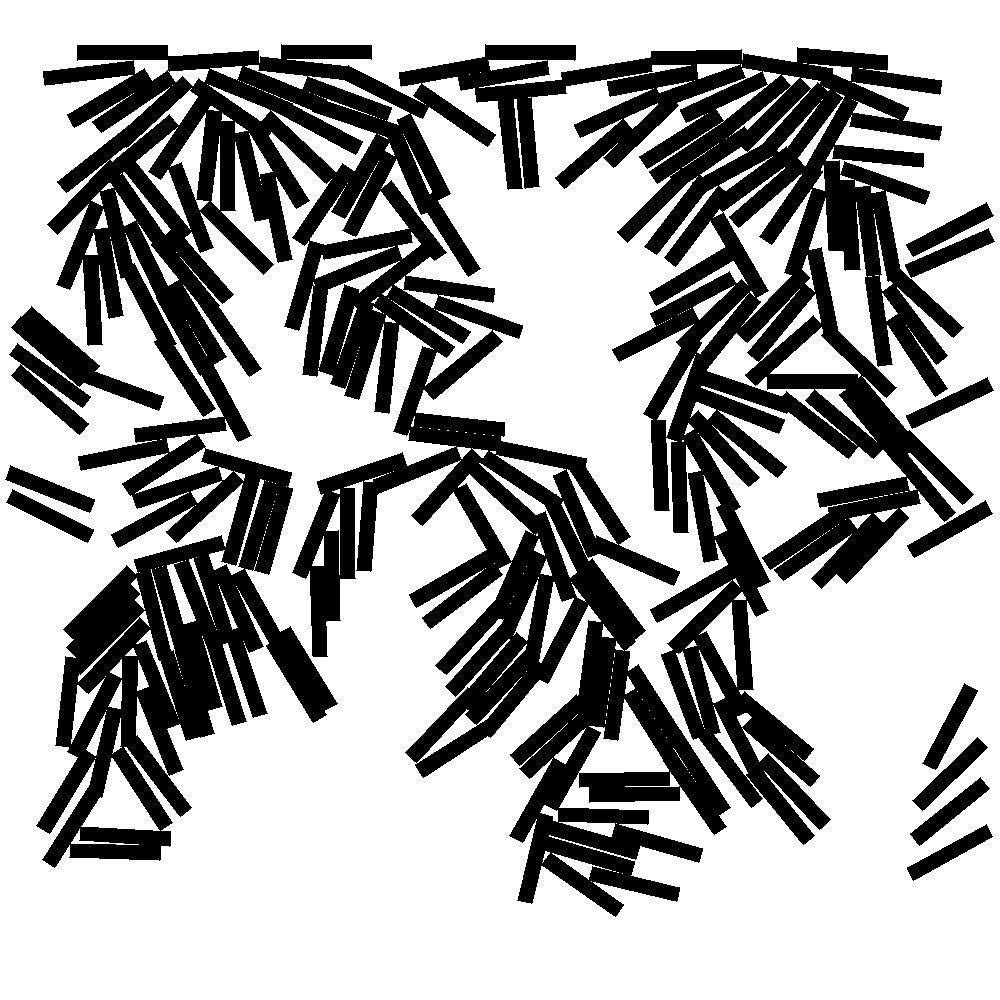
\includegraphics[width=\textwidth]{data/asp_thick.png}}
  \end{minipage}
  \hfill
  \begin{minipage}[t]{0.45\textwidth}
    \fbox{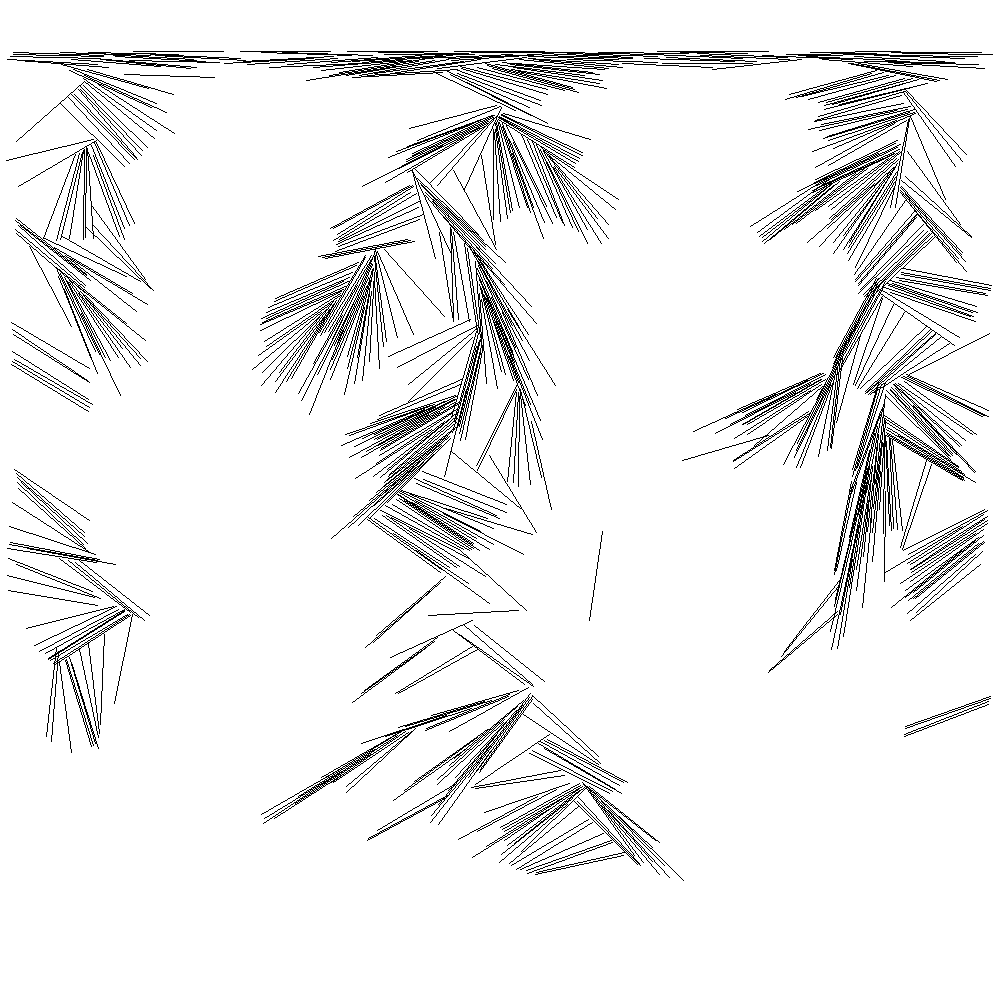
\includegraphics[width=\textwidth]{data/asp_thin.png}}
  \end{minipage}
  \caption{Comparison of lithium rods with equal length and an aspect ratio of 0.16 (left) and 0.01 (right) in water, picture shows end state after 1e7 MC iteration steps.}
  \label{fig:asp_length}
\end{figure}
HERE COMES TEXT ABOUT FIXED GRAVITY
